\section{Processi primari}
\subsection{Fornitura}
\subsubsection{Scopo}
Lo scopo del processo di fornitura è di determinare le procedure e le risorse necessarie allo svolgimento del progetto. Una volta comprese le richieste del proponente e aver stilato uno \textit{Studio di Fattibilità}, il processo può essere avviato con fine di soddisfare ognuna di queste richieste. Inoltre si deve stipulare e concordare con il proponente un contratto per la consegna del prodotto. Si passa dunque a determinare le procedure, le risorse necessarie, e si sviluppa un \textit{Piano di Progetto} che getterà le basi da perseguire fino alla consegna del materiale prodotto.
	Il processo di fornitura è composto dalle seguenti fasi:
	\begin{itemize}
		\item avvio;
		\item approntamento di risposte alle richieste;
		\item contrattazione;
		\item pianificazione;
		\item esecuzione e controllo;
		\item revisione e valutazione;
		\item consegna e completamento.
	\end{itemize}
	\subsubsection{Aspettative}
	Il gruppo intende mantenere un costante dialogo con il proponente, per avere un riscontro efficace sul lavoro svolto e instaurare un rapporto di collaborazione per quanto riguarda:
	\begin{itemize}
		\item determinare aspetti chiave per far fronte ai bisogni del proponente;
		\item stilare requisiti e vincoli sui processi;
		\item stimare le tempistiche di lavoro;
		\item promuovere una verifica continua;
		\item chiarire eventuali dubbi emersi;
		\item accordarsi sulla qualifica del prodotto.
	\end{itemize}
	\subsubsection{Descrizione}
	Questa sezione tratta le norme che i membri del gruppo \textit{8Lab Solutions} devono rispettare in tutte le fasi di progettazione, sviluppo e consegna del prodotto \textit{Soldino}, al fine di diventare fornitori nei confronti del proponente \textit{Red Babel} e dei committenti Prof. Tullio Vardanega e Prof. Riccardo Cardin.
	\subsubsection{Attività}
		\paragraph{Studio di Fattibilità} \mbox{}\\ \mbox{}\\
		\'E compito del responsabile di progetto organizzare riunioni tra i membri del gruppo al fine di permettere lo scambio di opinioni sui capitolati proposti.
		Lo \textit{Studio di Fattibilità}, redatto dagli analisti, indica per ogni capitolato\glo:
		\begin{itemize}
			\item \textbf{Informazioni generali}: vengono elencate le informazioni di base, come il nome del progetto, il proponente e il committente;
			\item \textbf{Descrizione e finalità del progetto}: viene fatta una presentazione del capitolato\glosp in generale, una descrizione delle caratteristiche principali richieste per il prodotto e viene definito l'obiettivo che si vuole raggiungere;
			\item \textbf{Tecnologie interessate}: viene fatto un elenco delle tecnologie richieste per lo svolgimento, che rientrano nel dominio tecnologico;
			\item \textbf{Aspetti positivi, criticità e fattori di rischio}: vengono esposte le considerazione fatte dal gruppo sugli aspetti positivi e sui fattori di rischio del capitolato\glo;
			\item \textbf{Conclusioni}: vengono esposte le ragioni per la quale il gruppo ha deciso di accettare o scartare il capitolato\glo.
		\end{itemize}
		\paragraph{Piano di Progetto} \mbox{}\\ \mbox{}\\
		Il responsabile, con l'aiuto degli amministratori, redige un \textit{Piano di Progetto} da seguire durante il corso del progetto. Questo documento contiene:
		\begin{itemize}
			\item \textbf{Analisi dei rischi}: vengono analizzati nel dettaglio i rischi che potranno presentarsi e vengono esposte le misure e le modalità attraverso le quali i rischi vengono contenuti o mitigati. Viene anche fornita la probabilità con la quale questi possono presentarsi e il livello di gravità per ciascuno;
			\item \textbf{Modello di sviluppo\glo}: viene descritto il modello di sviluppo\glosp che è stato scelto, indispensabile per la pianificazione;
			\item \textbf{Pianificazione}: vengono pianificate le attività da eseguire nelle diverse fasi del progetto e vengono stabilite le loro scadenze temporali;
			\item \textbf{Preventivo e consuntivo}: viene data una stima di lavoro necessaria per ciascuna fase proponendo così un preventivo per il costo totale del progetto. Viene anche tracciato, un consuntivo di periodo relativo all'andamento rispetto a ciò che è stato preventivato.
		\end{itemize}
		\paragraph{Piano di Qualifica} \mbox{}\\ \mbox{}\\
		I verificatori dovranno redigere un documento, detto \textit{Piano di Qualifica} contenente le strategie da adottare per garantire la qualità del materiale prodotto dal gruppo, e dei processi attuati. Il piano è così suddiviso:
		\begin{itemize}
			\item \textbf{Qualità di processo}: vengono identificati dei processi dagli standard, stabiliti degli obiettivi, escogitate delle strategie per attuarli e individuate le metriche per misurarli e controllarli;
			\item \textbf{Qualità di prodotto}: vengono identificati gli attributi più rilevanti per il prodotto, definiti degli obiettivi per raggiungerli e delle metriche per misurarli;
			\item \textbf{Specifiche dei test}: definiscono una serie di test attraverso i quali il prodotto passa per garantire che soddisfi i requisiti;
			\item \textbf{Standard di qualità}: vengono esposti gli standard di qualità scelti;
			\item \textbf{Valutazioni per il miglioramento:} vengono riportati i problemi e le relative soluzioni nel ricoprire un determinato ruolo e nell'uso degli strumenti scelti;
			\item \textbf{Resoconto delle attività di verifica:} per ogni attività si riportano i risultati delle metriche calcolate in forma di resoconto.
		\end{itemize}
		\subsubsection{Strumenti}
		Di seguito sono elencati gli strumenti utilizzati durante il processo di fornitura.
		\paragraph{Microsoft Excel} \mbox{}\\ \mbox{}\\
		Software della suite Microsoft Office per realizzare fogli elettronici. Usato per fare calcoli, produrre diagrammi, istogrammi e areogrammi, creare tabelle e grafici.
		\paragraph{Microsoft Project} \mbox{}\\ \mbox{}\\
		Per assistere i responsabili di progetto nella pianificazione, nell'assegnazione delle risorse, nella verifica del rispetto dei tempi, nella gestione dei budget e nell'analisi dei carichi di lavoro attraverso la creazioni di diagrammi di Gantt\glo, è stato utilizzato Microsoft Project. \\
		\centerline{\url{https://products.office.com/it-it/project/}}
		%PLACEHOLDER
		\begin{figure}[H]
			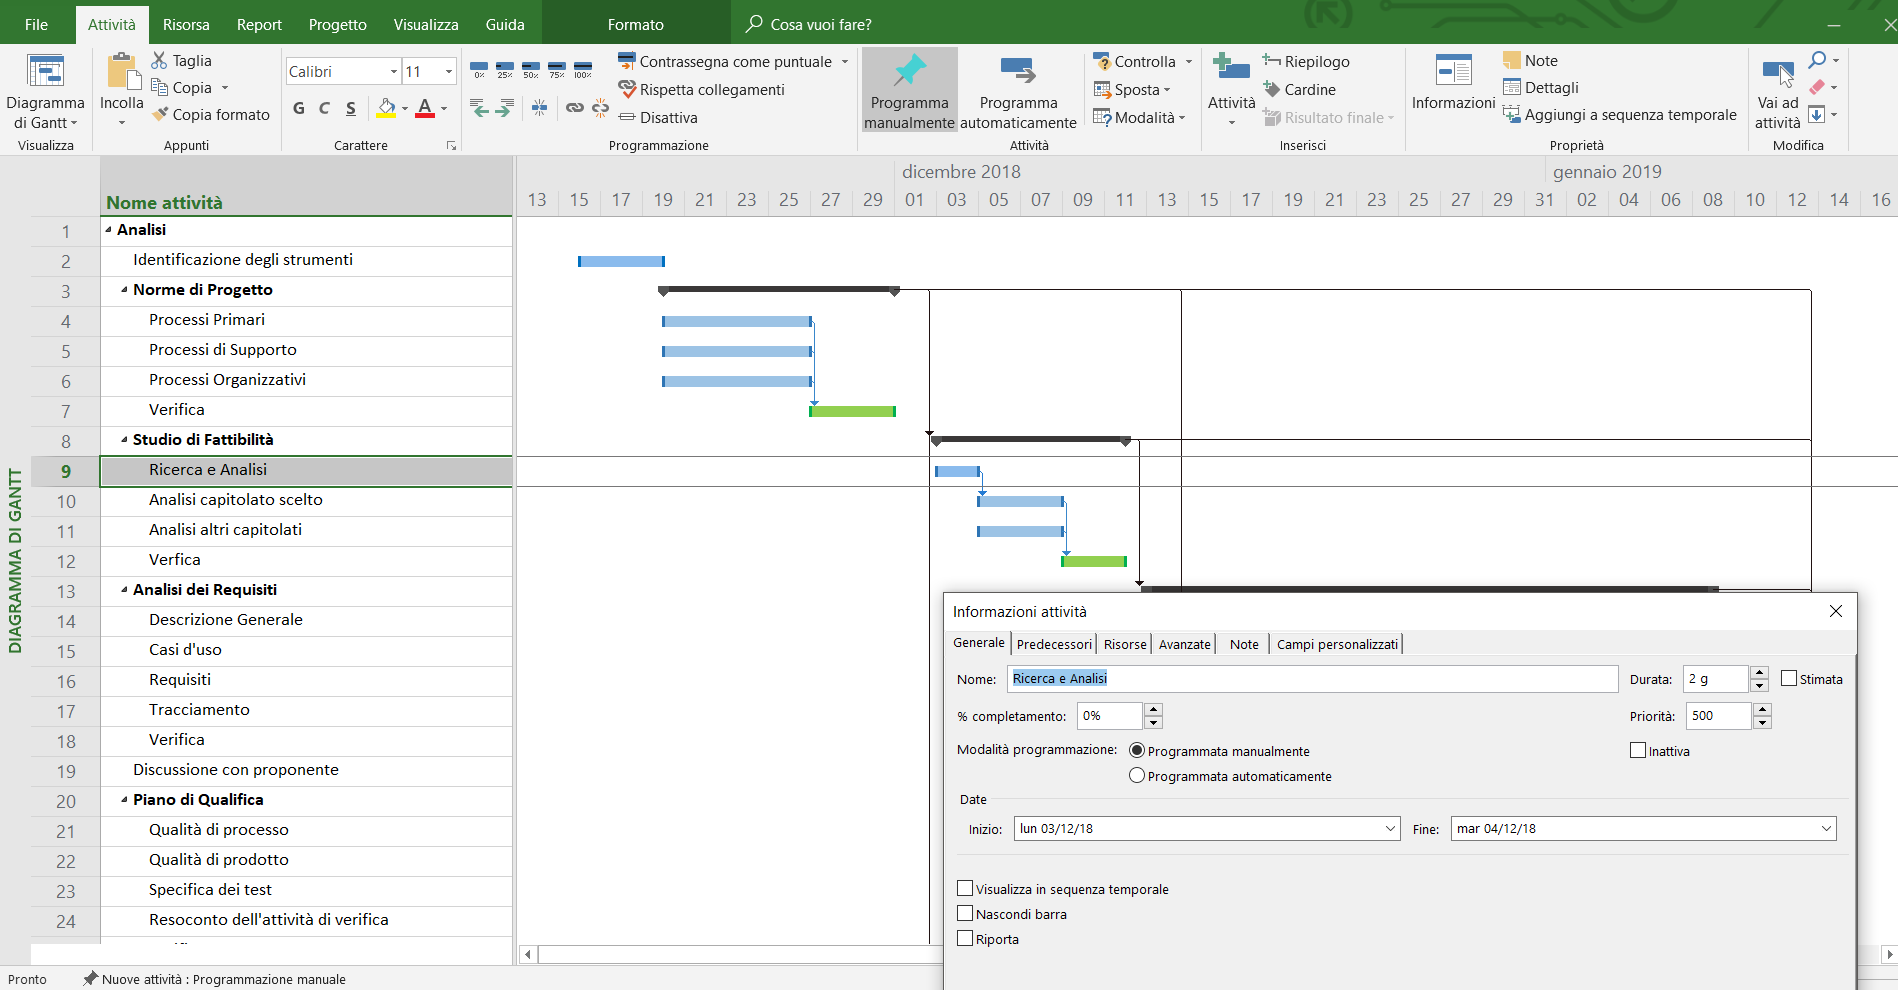
\includegraphics[width=0.99\linewidth]{res/images/projectS.png}
			\caption{Microsoft Project: Gantt}
		\end{figure} 
		\begin{comment}
		\textbf{(questa ultima sezione è da inserire nella fase successiva)}
		\subsubsection{Collaudo e consegna del prodotto}
		Al fine di consegnare il prodotto terminato il gruppo deve effettuare un collaudo in presenza del proponente e dei committenti. Precedentemente a questo test il gruppo deve assicurare correttezza, completezza e affidabilità per ogni parte del materiale consegnato, permettendo così che tutti i requisiti obbligatori siano soddisfatti e l'esecuzione dei test abbiano un esito positivo. In seguito al collaudo finale il responsabile di progetto consegna il prodotto su un supporto fisico.
		\end{comment}
     
\subsection{Sviluppo}
	\subsubsection{Scopo}
	Il processo contiene le attività e i compiti da svolgere, al fine di realizzare il prodotto finale richiesto dal proponente.
	\subsubsection{Aspettative}
	Le aspettative sono le seguenti:
	\begin{itemize}
		\item fissare gli obiettivi di sviluppo;
		\item fissare i vincoli tecnologici;
		\item fissare i vincoli di design;
		\item realizzare un prodotto finale che supera i test, che soddisfa i requisiti e le richieste del proponente.
	\end{itemize}
	\subsubsection{Descrizione}
	Il processo di sviluppo si articola in:
	\begin{itemize}
		\item \textit{Analisi dei Requisiti};
		\item Progettazione;
		\item Codifica.
	\end{itemize}
	\subsubsection{Attività}
		\paragraph{Analisi dei Requisiti} \mbox{}\\ \mbox{}\\
			\textbf{Scopo} \newline \newline
			Gli analisti hanno il compito di redigere il documento di
			\textit{Analisi dei Requisiti} che individua ed elenca dunque, i requisiti.
			Lo scopo dei requisiti è quello di:
			\begin{itemize}
				\item definire lo scopo del lavoro;
				\item fornire ai progettisti riferimenti precisi ed affidabili;
				\item fissare le funzionalità e i requisiti concordati col cliente;
				\item fornire  una  base  per  raffinamenti  successivi  al  fine  di  garantire  un miglioramento continuo del prodotto e del processo di sviluppo;
				\item fornire ai verificatori riferimenti per l'attività di controllo dei test;
				\item calcolare la mole di lavoro per tracciare dei riferimenti per un stima dei costi.
			\end{itemize}
			\textbf{Aspettative} \newline \newline
			Obiettivo dell'attività è la creazione della documentazione formale contenente tutti i
			requisiti richiesti dal proponente. \newline \newline
			\textbf{Descrizione} \newline \newline
			I requisiti si raccolgono secondo modalità predefinite:
			\begin{itemize}
				\item lettura del capitolato\glo, analisi e approfondimento dello stesso;
				\item confronto con il proponente;
				\item confronto tra membri del team di progetto;
				\item analisi di uno o più casi d'uso.  \\
			\end{itemize}
			\noindent
			\textbf{Casi d'uso} \newline \newline
			Rappresenta un diagramma che esprime un comportamento,
			offerto o desiderato, sulla base di risultati osservabili.
			La struttura dei casi d'uso è così suddivisa:
			\begin{itemize}
				\item codice identificativo;
				\item titolo;
				\item diagramma UML\glo;
				\item attori primari;
				\item attori secondari;
				\item descrizione;
				\item scenario principale;
				\item scenario alternativo (se presente);
				\item inclusioni(se presenti);
				\item estensioni(se presenti);
				\item specializzazioni(se presenti);
				\item precondizione;
				\item postcondizione. \\
			\end{itemize}
			\noindent
			\textbf{Codice identificativo dei casi d'uso} \newline \newline
			Il codice di ogni caso d'uso seguirà questo formalismo: \newline \newline
			\centerline{\textbf{UC[codice\_padre].[codice\_figlio]}} \\
			Dove:
			\begin{itemize}
				\item \textbf{codice\_padre}: numero che identifica univocamente i casi d'uso;
				\item \textbf{codice\_figlio}: numero progressivo che identifica i sottocasi. Può a sua volta includere altri livelli. \\
			\end{itemize}
			%\pagebreak
			%esempio di caso d'uso?(immagine)
			\noindent
			\textbf{Requisiti} \newline \newline
			Ogni requisito è composto dalla seguente struttura:
			\begin{itemize}
				\item \textbf{codice identificativo}: ogni codice identificativo è univoco e conforme alla seguente codifica: \\
				\centerline{\textbf{R[Importanza][Tipologia][Codice]}} \\ \\
				Il significato delle cui voci è:
				\begin{itemize}
					\item \textbf{Importanza}: ogni requisito può assumere uno dei seguenti valori:
					\begin{itemize}
						\item \textit{1}: requisito obbligatorio, ovvero irrinunciabile per gli stakeholder;
						\item \textit{2}: requisito desiderabile, ovvero non strettamente necessari ma a valore aggiunto riconoscibile;
						\item \textit{3}: requisito opzionale, ovvero relativamente utile oppure contrattabile più avanti nel progetto;	
					\end{itemize}
					\item \textbf{Tipologia}: ogni requisito può assumere uno dei seguenti valori:
					\begin{itemize}
						\item \textit{F}: funzionale;
						\item \textit{Q}: prestazionale;
						\item \textit{P}: qualitativo;
						\item \textit{V}: vincolo.
					\end{itemize}
					\item \textbf{Codice}: è un identificatore univoco del requisito in forma gerarchica padre/figlio.
				\end{itemize}
				\item \textbf{classificazione}: viene riportata l'importanza del requisito. Sebbene questa sia un'informazione ridondante ne facilita la lettura;
				\item \textbf{descrizione}: descrizione breve ma completa del requisito, meno ambigua possibile;
				\item \textbf{fonti}: ogni requisito può derivare da una o più tra le seguenti opzioni:
				\begin{itemize}
					\item \textit{capitolato\glo}: si tratta di un requisito individuato dalla lettura del capitolato\glo;
					\item \textit{interno}: si tratta di un requisito che gli analisti hanno ritenuto opportuno aggiungere;
					\item \textit{caso d'uso}: il requisito è estrapolato da uno o più casi d'uso. In questo caso deve essere riportato il codice univoco del caso d'uso;
					\item \textit{verbale}: si tratta di un requisito individuato in seguito ad una richiesta di chiarimento con il proponente. Tali informazioni sono riportate nei verbali in cui ogni requisito individuato è segnato da un codice presente nella tabella dei tracciamenti. \\
				\end{itemize}
			\end{itemize}

			\noindent{\textbf{UML}} \newline \newline
			I diagrammi UML\glosp devono essere realizzati usando la versione del linguaggio v2.0.

		\paragraph{Progettazione} \mbox{}\\ \mbox{}\\
			\textbf{Scopo} \newline \newline
			L'attività di progettazione definisce, in funzione dei requisiti specificati nel documento \textit{Analisi dei Requisiti}, le caratteristiche del prodotto software richiesto. Il compito di questa fase è di definire una soluzione del problema che sia soddisfacente per tutti gli stakeholder. La progettazione segue il procedimento inverso rispetto all'\textit{Analisi dei Requisiti} che divide il problema in parti per capirne completamente il dominio applicativo. La progettazione, infatti, rimette insieme le parti specificando le funzionalità dei sottosistemi in modo da ricondurre ad un'unica possibile soluzione. \newline \newline
			\textbf{Aspettative} \newline \newline
			Il processo ha come risultato la realizzazione dell’architettura del sistema. \newline \newline
			\textbf{Descrizione} \newline \newline
			Le parti principali sono due:
			\begin{itemize}
				\item \textbf{Technology baseline}: contiene le specifiche della progettazione ad alto livello del prodotto e delle sue componenti, l'elenco dei diagrammi UML\glosp che saranno utilizzati per la realizzazione dell'architettura e i test di verifica;
				\item \textbf{Product baseline}: dettaglia ulteriormente l'attività di progettazione, integrando ciò che è riportato nella Technology baseline. Inoltre definisce i test necessari alla verifica.
			\end{itemize}
			\textbf{Technology baseline} \newline \newline
			Redatta dal progettista, dovrà includere:
			\begin{itemize}
				\item \textbf{Diagrammi UML\glo}:
				\begin{itemize}
					\item diagrammi delle classi;
					\item diagrammi dei package;
					\item diagrammi di attività;
					\item diagrammi di sequenza.
				\end{itemize}
				\item \textbf{Tecnologie utilizzate}: devono essere descritte le tecnologie adottate specificandone l'utilizzo nel progetto, i vantaggi e gli svantaggi;
				\item \textbf{Design pattern\glo}: devono essere descritti i design pattern\glosp utilizzati per realizzare l'architettura. Ogni design pattern\glosp deve essere accompagnato da una descrizione ed un diagramma, che ne esponga il significato e la struttura;
				\item \textbf{Tracciamento delle componenti}: ogni requisito deve riferirsi al componente che lo soddisfa;
				\item \textbf{Test di integrazione}: l'unione delle parti, intese come classi di verifica, permette di verificare che ogni componente del sistema funzioni nella maniera voluta.
			\end{itemize}
			\textbf{Product baseline} \newline \newline
			A carico del progettista c'è anche la Product baseline che si sofferma su diversi aspetti tra i quali:
			\begin{itemize}
				\item \textbf{definizione delle classi}: ogni classe deve essere descritta in modo da spiegarne in maniera esaustiva lo scopo e le funzionalità, evitando ridondanze;
				\item \textbf{tracciamento delle classi}: ogni requisito deve essere tracciato in modo da garantire che per ognuno esista una classe che lo soddisfi. Questa operazione è fondamentale per permettere di risalire alle classi ad esso associate;
				\item \textbf{test di unità}: devono essere definiti al fine di verificare che le parti funzionino individualmente nel modo stabilito.
			\end{itemize}
		\paragraph{Codifica} \mbox{}\\ \mbox{}\\
			\textbf{Scopo} \newline \newline
			Questa attività ha come scopo quello di normare l'effettiva realizzazione del prodotto software richiesto. In questa fase si concretizza la soluzione attraverso la programmazione. I programmatori dovranno attenersi a queste norme durante la fase di programmazione ed implementazione. \newline \newline
			\textbf{Aspettative} \newline \newline
			Obiettivo dell'attività è la creazione di un prodotto software conforme alle richieste	prefissate con il proponente.
			L'uso di norme e convenzioni in questa fase, è fondamentale per permettere la generazione di codice leggibile ed uniforme,  agevolare le fasi di manutenzione,  verifica e validazione e migliorare la qualità di prodotto. \newline \newline
			\textbf{Descrizione} \newline \newline
			La scrittura del codice dovrà rispettare quanto stabilito nella documentazione di prodotto. Dovrà perseguire gli obiettivi di qualità definiti all'interno del documento \textit{Piano di Qualifica v1.0.0} per poter garantire una buona qualità del codice. \newline \newline
			\textbf{Stile di codifica} \newline \newline
			Al fine di garantire uniformità nel codice del progetto, ciascun membro del gruppo è
			tenuto a rispettare le seguenti norme:
			\begin{itemize}
				\item \textbf{Indentazione}: i blocchi innestati devono essere correttamente indentati, usando per ciascun livello di indentazione quattro (4) spazi (fanno eccezione i commenti). Al fine di assicurare il rispetto di questa regola si consiglia di configurare adeguatamente il proprio editor o IDE;
				\item \textbf{Parentesizzazione}: è richiesto di inserire le parentesi di delimitazione dei costrutti in linea e non al di sotto di essi;
				\item \textbf{Scrittura dei metodi}: è desiderabile, ove possibile, mantenere i metodi brevi(poche righe di codice);
				\item \textbf{Univocità dei nomi}: classi, metodi, variabili devono avere un nome univoco	ed esplicativo al fine di evitare ambiguità e incomprensione;
				\item \textbf{Classi}: i nomi delle classi devono iniziare sempre con una lettera maiuscola;
				\item \textbf{Costanti}: i nomi delle costanti devono essere scritte usando solo maiuscole;
				\item \textbf{Metodi}: i nomi dei metodi devono iniziare con una lettera minuscola. Nel caso
				siano composti da più parole, quelle successive devono iniziare con una lettera maiuscola (CamelCase\glo{});
				\item \textbf{Lingua}: il codice, come anche i commenti, deve essere scritto in lingua inglese.
			\end{itemize}
			Una parte del front end\glosp è normata dalla "Airbnb JavaScript style guide", il cui uso è implementato attraverso ESLint\glo. \newline \newline
			%\subparagraph{Intestazione} \mbox{}\\
			\textbf{Ricorsione} \newline \newline
			L'uso della ricorsione va evitato quanto più possibile in  quanto  potrebbe
			indurre  ad  una  maggiore  occupazione  di  memoria  rispetto  a  soluzioni
			iterative.
	\subsubsection{Strumenti}
	Di seguito sono elencati gli strumenti utilizzati dal gruppo durante il progetto per il processo di sviluppo.
		\paragraph{ESLint} \mbox{}\\ \mbox{}\\
		Utilità open-source per scrivere codice JavaScript secondo regole di codifica predeterminate. Esegue segnalazioni su patterns presenti nel codice ECMAScript/JavaScript.
		\paragraph{PragmaDB} \mbox{}\\ \mbox{}\\
		Programma usato per il tracciamento dei requisiti, fondamentale dunque per la stesura del documento \textit{Analisi dei Requisiti v1.0.0}. \newline
		\centerline{\url{https://github.com/StefanoMunari/PragmaDB}}
		\paragraph{Draw.io} \mbox{}\\ \mbox{}\\
		Per la produzione di diagrammi UML\glosp viene utilizzato Draw.io in quanto offre molte agevolazioni per la produzione veloce dei diagrammi e risulta semplice da usare. \newline
		\centerline{\url{https://www.draw.io/}}
		\begin{figure}[H]
			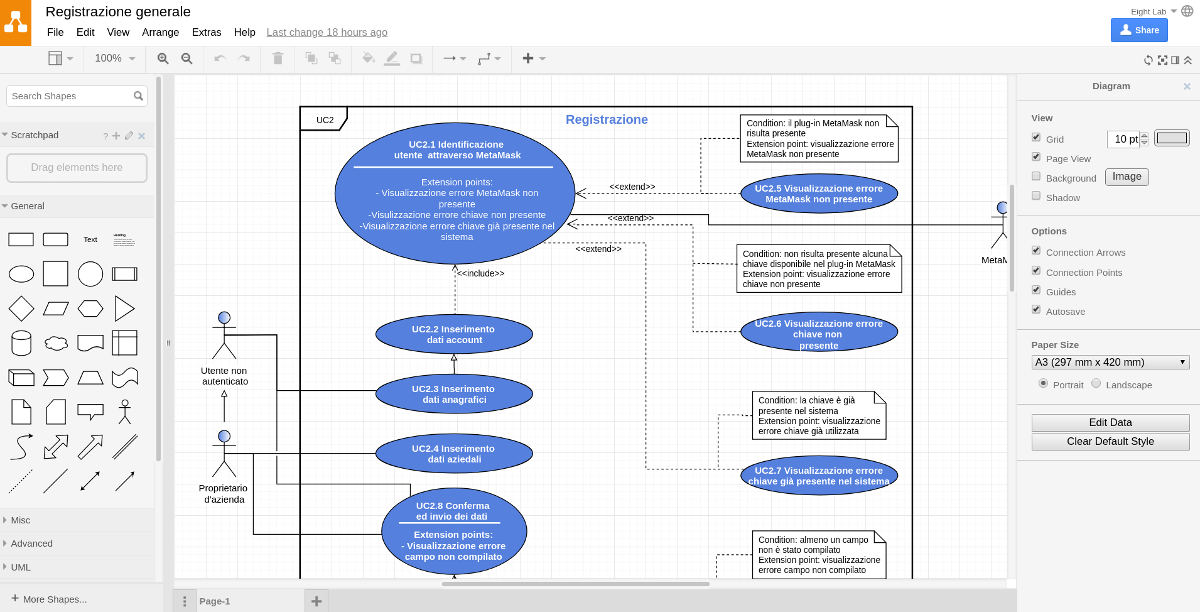
\includegraphics[width=0.99\linewidth]{res/images/drawio.jpg}
			\caption{Software per la creazione di diagrammi online}
		\end{figure} 
		\paragraph{IntelliJ IDEA} \mbox{}\\ \mbox{}\\
		IntelliJ IDEA viene utilizzato per la codifica in Java e JavaScript. Questo IDE offre piena compatibilità con Linux, Windows, macOS, oltre ad essere un potente editor con molte funzionalità integrate. \newline
		\centerline{\url{https://www.jetbrains.com/idea/}}
		\begin{comment}
			\begin{figure}[H]
			\includegraphics[width=0.99\linewidth]{res/images/""}
			\caption{Software per la codifica}
			\end{figure} 
		\end{comment}
